\chapter{\label{ch:4-strategy}Analytical strategy}

\section{Data}
The English Longitudinal Study of Ageing (ELSA) was initiated in 2002. It is a large scale longitudinal panel study of older people aged 50 and above and their partners, residing in private households in England. The initial cohort was drawn from households that had previously participated in the Health Survey for England (HSE) between 1998 and 2001. To maintain the study's representativeness and relevance, the sample has been periodically refreshed during the third, fourth, sixth, seventh, and ninth waves. 

ELSA conducted two-yearly interviews, referred to as ``waves”, to track changes in their health, economic and social circumstances. This structured approach allows for a detailed longitudinal analysis of ageing dynamics within the population (NatCen Social Research, 2020). Ethical approval for the ninth and tenth waves of ELSA was granted by the South Central - Berkshire Research Ethics Committee on 10th May 2018 (17/SC/0588) and 22nd March 2021 (21/SC/0030) respectively (ELSA project, 2024). For this thesis, ELSA data (40th edition, 6 February 2024) was obtained through the UK Data Service website under an End User Licence agreement (Banks et al., 2024). 

\section{Sample selection}
This thesis draws on data from Wave 9 and 10 of ELSA. These two waves are selected because they contain information on respondents' Internet use, which has been included in ELSA starting from Wave 9 (Vidiasratri \& Bath, 2022). The interview fieldwork was carried out between June 2018 and July 2019 for Wave 9 and between October 2021 and July 2022 for Wave 10. In other words, Wave 9 was conducted prior to the COVID-19 pandemic, whereas Wave 10 was conducted during the pandemic (NatCen Social Research, 2020, 2022). 

The first research question draws on data from Wave 10 only. The sample selection process is outlined as follows:

\begin{enumerate}
    \item The initial sample consists of all respondents from Wave 10.
    \item Remove respondents missing key information due to the non-release of IFS derived variables dataset \footnote{The IFS derived variable dataset, compiled by researchers from the Institute for Fiscal Studies, serves as a valuable supplement to the core ELSA dataset (IFS, 2022).} \footnote{This information missingness arises because, at the time of this thesis, only the first release of Wave 10 data was available, which includes just the core data and pension grid data. Many additional datasets that are typically very useful, such as the financial derived variables and IFS derived variables, have not yet been released. Crucial information like ethnicity and educational attainment, typically found in the IFS derived variables dataset, is absent for some respondents at Wave 10. Consequently, this study has had to manually derive these variables using data from previous waves, resulting in this information missingness.}.
    \item Remove respondents who were ineligible for the self-completion questionnaire, as it includes questions on Internet usage that are necessary for this study.
    \item Remove respondents residing in institutions (e.g. care homes), because the relationship between digital literacy and health may differ fundamentally for this group, given that they can get help with access to the Internet and their health is centrally managed by the institution.
    \item For similar reasons, remove respondents who received formal care at home, such as those assisted by home care workers.
    \item For similar reasons, remove respondents who received informal care at home (e.g. from family members or other non-professionals).
    \item Remove respondents who did not have Internet access at home to ensure the accuracy of the constructed digital literacy index. A more detailed explanation will be provided in Section 4.3.1.2.
\end{enumerate}

The specific reductions in sample size at each step are detailed in Appendix. The initial sample size from Wave 10 was 7,586, and after the sample selection process, the sample size is 4,017.

The second research question draws on data from both Wave 9 and 10 as the nature of this question requires a comparison between two time points. The sample selection process is outlined as follows:

\begin{enumerate}
    \item The initial sample consists of the intersection (i.e. inner join) of respondent from Wave 9 and 10.
    \item Remove respondents who were ineligible for the self-completion questionnaire in either wave, as it includes questions on Internet usage that are necessary for this study.
    \item Remove respondents residing in institutions (e.g. care homes) in either wave, because the relationship between digital literacy and health may differ fundamentally for this group, given that they can get help with access to the Internet and their health is centrally managed by the institution.
    \item For similar reasons, remove respondents who received formal care at home in either wave, such as those assisted by home care workers.
    \item For similar reasons, remove respondents who received informal care at home in either wave (e.g. from family members or other non-professionals).
    \item Remove respondents who did not have Internet access at home in either wave to ensure the accuracy of the constructed digital literacy index. A more detailed explanation will be provided in Section 4.3.1.2.
\end{enumerate}

It should be noted that the sample presented here does not correspond precisely to the sample used in the final analysis. This is because subsequent analytical strategies (described in Section 4.4 and Section 4.6) involve steps that lead to further reductions in sample size. This section merely presents the preliminary sample that meets the initial criteria for inclusion in the analysis. Detailed information on the final sample size is available in the tables and figures in Section 5.

\section{Variables}

\subsection{Explanatory variable}
The explanatory variable in this study is digital literacy. However, ELSA does not directly collect data on respondents' digital literacy levels. Therefore, this study constructs a new variable representing digital literacy from the available data on respondents' Internet usage within ELSA. In measurement terms, this newly created variable is referred to as an ``index" — in this case, a digital literacy index. The variables used to build this index are referred to as ``features" or the ``feature set". To construct the digital literacy index, this study utilises principal component analysis (PCA). This section firstly explains the rationale for selecting the feature set, and then describe how the PCA methodology is implemented to construct the digital literacy index.

To clarify, the digital literacy index derived by PCA is a continuous variable as it is the score of the first principal component (more details will be provided in Section 4.3.1.2). For analysis purposes, this digital literacy index is then dichotomised by taking the lower and the upper quartile. This binary variable categorises respondents into low and high levels of digital literacy and is used as the explanatory variable in the study. 

\subsubsection{Selection of feature set}
Digital literacy is defined as the ability to use ICTs to find, evaluate, create, and communicate information (van Kessel, Wong, et al., 2022). As analysed in Section 2.3.1, van DijK (2005, p. 21) proposes that digital literacy comprises two key dimensions: instrumental and informational. The instrumental dimension pertains to hardware literacy, focusing on an individual's ability to operate devices such as mobile phones, tablets, and computers to connect to the Internet. The informational dimension, on the other hand, pertains to software literacy. It focuses on individuals' ability to effectively search, select, process, and utilise information from an abundance of sources to accomplish relevant tasks. Additionally, acknowledging the prevalence of using frequency of Internet usage as a proxy in existing studies, this study incorporates this metric as well. Therefore, the feature set selected for constructing the digital literacy index in this study encompasses frequency of Internet usage, hardware literacy, and software literacy, aiming to provide a holistic assessment of digital literacy's multiple facets.

Frequency of Internet usage assesses how often respondents use the Internet. In ELSA, it is a self-reported measure on a six-point ordinal scale: 1 (daily), 2 (at least once a week), 3 (at least once a month), 4 (at least once every three months), 5 (less than every three months), 6 (never). For analysis purposes, frequency is treated as a continuous variable in the construction of the digital literacy index.

In ELSA, hardware literacy is measured through a series of questions which ask respondents whether they use specific devices to access the Internet (see Table \ref{tab:hardware} for a detailed list of questions). Responses to these questions are coded as binary variables: 1 for affirmative and 0 for negative. Due to differences in survey design, there are some variations between the hardware literacy questions included in Wave 9 and 10. 

\begin{table}[h!]
    \centering
    \caption{Hardware --- Devices used to access the Internet}
    \label{tab:hardware}
    \begin{tabular}{ll}
        \toprule
        Wave 9 (N = 6) & Wave 10 (N = 5) \\
        \midrule
        Desktop & Desktop \\
        Laptop & Laptop \\
        Tablet & Tablet \\
        Smartphone & Smartphone \\
        Other devices & Other devices \\
        Do not use any device & \\
        \bottomrule
    \end{tabular}
\end{table}

In ELSA, software literacy is measured through a series of questions which ask respondents whether they engage in certain online activities (see Table \ref{tab:software} for a detailed list of questions). Responses to these questions are coded as binary variables: 1 for affirmative and 0 for negative. Due to differences in survey design, there are some variations between the software literacy questions included in Wave 9 and 10.

\begin{table}[h!]
    \centering
    \caption{Software --- Activities engaged in online}
    \label{tab:software}
    \begin{tabular}{ll}
        \toprule
        Wave 9 (N = 16) & Wave 10 (N = 21) \\
        \midrule
        Emails & Emails \\
        Video calls & Video calls \\
        Finding information (learning) & Finding information \\
        Finding information (health) & \\
        Finances & Finances \\
        Shopping & Shopping \\
        Selling & Selling \\
        Social networking & Social networking \\
        Creating content & \\
        News & News \\
         & TV/radio \\
        Music & Music \\
        Games & Games \\
         & E-books \\
        Job application & Job application \\
        Government services & Government services \\
         & Checking travel times \\
         & Satellite navigation \\
         & Buying public transport tickets \\
         & Booking a taxi \\
         & Finding local amenities \\
         & Controlling household appliances \\
        Other online activities & \\
        No online activities & No online activities \\
        \bottomrule
    \end{tabular}
\end{table}

It is important to note that, within the ELSA survey design, respondents who answered ``never" to the frequency of Internet usage question were not prompted to answer subsequent questions about hardware or software literacy. Consequently, their responses for hardware and software are recorded as missing/not applicable. To avoid losing valuable data, this study presumes that these respondents do not use any devices to access the Internet, and hence imputes all hardware literacy responses as zero except for a ``do not use any device" variable set to one. Similarly, this study presumes that they do not engage in any online activities, and hence imputes all software literacy responses as zero except for a ``no online activities" variable set to one. This imputation should not cause too much concern given that these respondents never use the Internet.

\subsubsection{Principal component analysis}
AAlthough ELSA does not directly measure digital literacy, it provides a comprehensive feature set that encapsulates the core aspects of digital literacy. This situation strongly supports the use of Principal Component Analysis (PCA) to construct the target measure. PCA is advantageous here as it reduces the feature set into a smaller number of representative components that account for the majority of the variability in the original data, thereby providing a succinct summary (James et al., 2023, p. 504). 

PCA is an unsupervised machine learning technique that reduces the dimensionality of a dataset while retaining as much variability as possible. In a scenario where there are $n$ observations and $p$ features, each observation can be considered to reside within a $p$-dimensional space. However, not all dimensions contribute equally to the dataset's structure. PCA aims to identify the most "interesting" dimensions, where interest is quantified by the degree of variance among the observations along each dimension (James et al., 2023, p. 505). These dimensions are known as "principal components".

A PCA applied to $p$ features yields $p$ principal components. Each principal component is a linear combination of the $p$ original features:

\begin{equation}
    \label{eq:pca_loadings}
    Z = \phi_{1}X_1 + \phi_{2}X_2 + \ldots + \phi_{p}X_p
\end{equation}

and the variance explained by the $i^{th}$ principal component is:

\begin{equation}
    \label{eq:pca_variance}
    \frac{1}{n} \sum_{i=1}^{n}Z_{im}^2 = \frac{1}{n} \sum_{i=1}^{n} \left( \sum_{j=1}^{p} \phi_{jm}X_{ij} \right)^2
\end{equation}

Mathematically, it can be shown that the sum of variance explained by each principal component is equal to the total variance of the feature set:

\begin{equation}
    \label{eq:pca_total_variance}
    \sum_{j=1}^{p} \frac{1}{n} \sum_{i=1}^{n}Z_{im}^2 = \sum_{j=1}^{p} \frac{1}{n} \sum_{i=1}^{n}X_{ij}^2
\end{equation}

The coefficients $\phi_{i1}, \phi_{i2}, \ldots, \phi_{ip}$ are known as the loadings of the principal component. To ensure meaningful interpretation and prevent arbitrarily large variance, these loadings are normalised so their sum of squares equals one (James et al., 2023, p. 505). The $Z$ is known as the score of the principal component.

The algorithm \footnote{It is crucial to standardise the features before performing PCA. This is because PCA seeks to identify the derived variables that capture the most variance in the feature set. Without standardisation, the principal components would mostly be driven by the variable with the largest variance, causing bias in the analysis (James et al., 2023, p. 512).} of deriving the first principal component (PC1) involves identifying the loadings (i.e., $\phi_{11}, \phi_{12}, \ldots, \phi_{1p}$) such that their corresponding score (i.e., $Z$) maximises the sample variance, under the constraint that the sum of the squares of the loadings equals one (James et al., 2023, p. 506). This optimisation problem is mathematically expressed as: 

\begin{equation}
    \label{eq:pca_algorithm}
    \textnormal{maximise}_{\phi_{11}, \ldots, \phi_{p1}} \left\{ \frac{1}{n} \sum_{i=1}^{n} \left( \sum_{j=1}^{p} \phi_{j1} X_{ij} \right)^2 \right\} \textnormal{subject to} \sum_{j=1}^{p} \phi_{j1}^2 = 1
\end{equation}

The principal components are calculated sequentially. Once PC1 is established, the second principal component (PC2) is determined as the loadings (i.e., $\phi_{21}, \phi_{22}, \ldots, \phi_{2p}$) that yield the maximum variance among all possible loadings that are uncorrelated (i.e. orthogonal) to PC1. In essence, PC2 captures the maximum residual variance of the feature set that is unexplained by PC1. This iterative process continues until the $p^{th}$ principal component is identified (James et al., 2023, p. 507).

Given that a total of $p$ principal components will be identified, a critical question arises: how many principal components are sufficient to capture the essential variation, which is presumed to represent digital literacy, within the feature set? There are three commonly accepted rules of thumb: (i) principal components should be selected in sequence since each one is constructed based on the residual variance unexplained by its predecessors; ii) the selected principal component(s) should appear as upwards outliers in the screeplot; iii) the selected principal component(s) should at least explain 20\% of the total variance (Zelterman, 2015, p. 212). Therefore, this study will select principal component(s) that meet these criteria, and the score ($Z$) of these principal components is expected to be a valid index for digital literacy.

Finally, to obtain the explanatory variable for the first research question, the score of the selected principal components is dichotomised. To ensure an efficient and meaningful classification, respondents scoring in the lower quartile (i.e., the bottom 25\%) are categorised as having low digital literacy, coded as 0, and those scoring in the upper quartile (i.e., the top 25\%) are categorised as having high digital literacy, coded as 1. This method is preferred over a simple median split, which tends to drag each group's digital literacy level towards the central point, potentially diluting the contrast between them and thus biasing the analysis results by underestimating the differences.

A potential concern with this PCA approach is that variations in the feature set might not solely arise from differences in digital literacy levels but could also be influenced by differences in the access to the Internet. The lack of Internet access can affect frequency of Internet usage, hardware literature, and software literacy in a manner very similar to low digital literacy, therefore resulting in very similar loadings on the identified principal components. To address this, as noted in Section 4.2, respondents without Internet access at home were excluded from the analysis. This adjustment ensures that the selected principal component(s) only reflects variations in digital literacy levels among respondents.


\subsection{Outcome variables}
The outcome variables in this study span three dimensions of health: self-rated health, physical health, and mental health. Altogether, ten health outcomes are examined to provide a comprehensive assessment of an individual's overall health status.

\subsubsection{Self-rated health}
Self-rated health, as the name suggests, measures how respondents rate their own health in general. It is measured on a five-point ordinal scale: 1 (excellent), 2 (very good), 3 (good), 4 (fair), 5 (poor). For analysis purposes, self-rated health is treated as a continuous variable.

\subsubsection{Physical health}
In this study, physical health is quantified through disease presence, which reflects the more objective aspects of health as opposed to self-rated health. Disease presence serves as a reliable objective metric because it can be consistently and accurately measured across the population (Thacker et al., 2006). Specifically, six diseases — three cardiovascular and three non-cardiovascular chronic conditions — are selected to ensure comprehensive coverage of various physiological systems in the human body (Seplaki et al., 2006). All diseases are measured on a binary scale, with 1 indicating the presence of the disease and 0 indicating its absence.

The three cardiovascular diseases examined are high blood pressure, high cholesterol, and diabetes. ELSA provides direct information on whether respondents currently have high blood pressure and high cholesterol, which this study directly employs. However, ELSA does not collect information regarding respondents' current diabetes status, so this study instead uses information on whether respondents have ever been diagnosed with diabetes. The potential rationale for ELSA not collecting current diabetes status is that, as of the time of this thesis, diabetes remains incurable (Diabetes UK, 2024). Therefore, it is appropriate to use ``ever diagnosed” as a reliable proxy because respondents who have been diagnosed with diabetes are very likely to still have the condition at the current wave.

The three non-cardiovascular diseases examined are arthritis, asthma, and cancer. ELSA provides direct information on whether respondents currently have these three conditions, and this study employs this information directly.

It is important to note differences in how disease presence data is recorded between Wave 9 and Wave 10. In Wave 9, the data differentiate between respondents who had the disease prior to Wave 9 and those for whom the disease was newly reported at Wave 9. A union operation (i.e., either A or B) is necessary to combine these two groups before the data can be used in the analysis. In Wave 10, the data regarding disease presence are already consolidated and can be used directly.

\subsubsection{Mental health}
In this study, mental health is quantified through the presence of mental health problems, which again reflects the more objective aspects of health as opposed to self-rated health. Specifically, three mental health problems — depression, anxiety disorder and mood swings - are selected because they are among the most common mental health problems worldwide, affecting a significant portion of the population (World Health Organization, 2023). 

Depression is measured as a depression score from the eight-item version of the Centre for Epidemiologic Studies Depression (CES-D) Scale, which is widely used in older population and has been validated for both reliability and validity (White et al., 2016). The CES-D scale includes questions that evaluate the respondents’ emotional feelings and somatic symptoms experienced over the past week (see Table \ref{tab:cesd} for a comprehensive list of the questions). The scoring of the CES-D scale involves adding the total number of affirmative responses for negatively worded items and the total number of negative responses for positively worded items. Therefore, the depression score ranges from 0 to 8, with higher scores indicating greater depressive symptoms. For analysis purposes, this depression score is treated as a continuous variable.

\begin{table}[h!]
    \centering
    \caption{Eight-item version of the CES-D scale}
    \label{tab:cesd}
    \begin{threeparttable}
        \begin{tabular}{lll}
            \toprule
            Item & Description & Positively worded \\
            \midrule
            1 & Whether felt depressed much of the time & No \\
            2 & Whether felt everything did was an effort & No \\
            3 & Whether felt sleep was restless & No \\
            4 & Whether was happy much of the time & Yes \\
            5 & Whether felt lonely much of the time & No \\
            6 & Whether enjoyed life much of the time & Yes \\
            7 & Whether felt sad much of the time & No \\
            8 & Whether could not get going much of the time & No \\
            \bottomrule
        \end{tabular}
        \begin{tablenotes}
            \footnotesize
            \item Notes: A positively worded item is one where an affirmative response indicates lower levels of depression, while a negative response indicates higher levels of depression.
        \end{tablenotes}
    \end{threeparttable}
\end{table}

Anxiety disorder is measured through whether the respondent has ever been diagnosed with anxiety disorder. It is a binary variable with 1 indicating ever diagnosed and 0 indicating never diagnosed. Similar to diabetes, anxiety disorder cannot be clinically cured as of the time of this thesis (NHS, 2022). Given that ELSA does not collect information on respondents' current anxiety disorder status, it is appropriate to use ``ever diagnosed” as a reliable proxy.

Mood swings is measured through whether the respondent has ever been diagnosed with mood swings. It is a binary variable with 1 indicating ever diagnosed and 0 indicating never diagnosed. Similar to diabetes, mood swings cannot be clinically cured as of the time of this thesis (Farrell, 2010, p. 28). Given that ELSA does not collect information on respondents' current mood swings status, it is appropriate to use ``ever diagnosed” as a reliable proxy.

\subsection{Control variables}
As discussed in Section 2.3.2, omitted variable bias significantly affects the relationship between digital literacy and health. Following an extensive review of the existing literature to identify key confounders (Hall et al., 2015; He et al., 2022; J. W. Hong et al., 2023; Mitchell et al., 2019), this study has selected the following twelve variables as controls.

\begin{itemize}[wide=0pt, leftmargin=*, labelwidth=0pt, labelindent=\parindent, itemindent=0pt]
    \item Age \\
    Age is measured in years as a continuous variable. In ELSA, ages 90 and over are collapsed and recoded as 99 to protect confidentiality. To prevent this from biasing the results, this study recodes ages 90 and over as missing.
    \item Gender \\
    Gender is a binary variable, with 1 indicating female and 0 indicating male.
    \item Marital status \\
    Marital status is a six-level categorical variable: single, married, remarried, separated, divorced and widowed.
    \item Ethnicity \footnote{As noted in Section 4.2, the IFS derived variables dataset for Wave 10 has not been released, leading to missing information on some respondents' ethnicity and educational attainment. As a result, this study has manually derived these data using information from Wave 9.}\label{fn:ifs} \\
    Ethnicity is a binary variable, with 1 indicating non-White and 0 indicating White.
    \item Educational attainment \\
    Educational attainment is represented by two variables. \\
    Age left full-time education: This is an eight-point ordinal variable representing the age at which respondents completed their full-time education: 1 (not yet finished), 2 (never went to school), 3 (14 or under), 4 (left at 15), 5 (left at 16), 6 (left at 17), 7 (left at 18), and 8 (19 or over). According to ELSA documentation, respondents who reported “not yet finished” should be classified as not applicable (i.e. missing), as they should not be in full-time education while participating in ELSA. For analytical purposes, age left full-time education is treated as a continuous variable. \\
    Highest educational level: This is a seven-level categorical variable that describes the highest level of education achieved by respondents. The categories are: degree or equivalent, higher education below degree, A level or equivalent, O level or equivalent, CSE or equivalent, foreign/other qualification, and no qualification. This variable is not treated as continuous due to the difficulty in assigning a clear hierarchical order to the categories, particularly for ``foreign/other qualification" which does not easily fit into a traditional educational ranking system.
    \item Employment status \\
    Employment status is a binary variable, with 1 indicating the respondent is in paid employment and 0 indicating the respondent is not in paid employment. 
    \item Household income \\
    Household income is measured using deciles of the respondent's pre-tax total household income, which is a continuous variable ranging from 0 to 9. Here, 0 indicates the lowest income decile and 9 the highest. In the ELSA core dataset, individual income types are listed separately (as illustrated in Figure \ref{fig:household_income}). The IFS derived variables dataset consolidates these individual income types into a single variable representing the total household income, and then calculates its corresponding deciles \footnote{This consolidated decile measure is directly utilised for Wave 9. However, as noted earlier, the IFS derived variables dataset for Wave 10 has not yet been released. Consequently, this study follows the procedure outlined in Figure \ref{fig:household_income} to manually derive the household income for Wave 10 and then calculate its corresponding deciles.}. 

    \begin{figure}
        \centering
        \caption{Structure of household income in IFS derived variables dataset}
        \label{fig:household_income}
        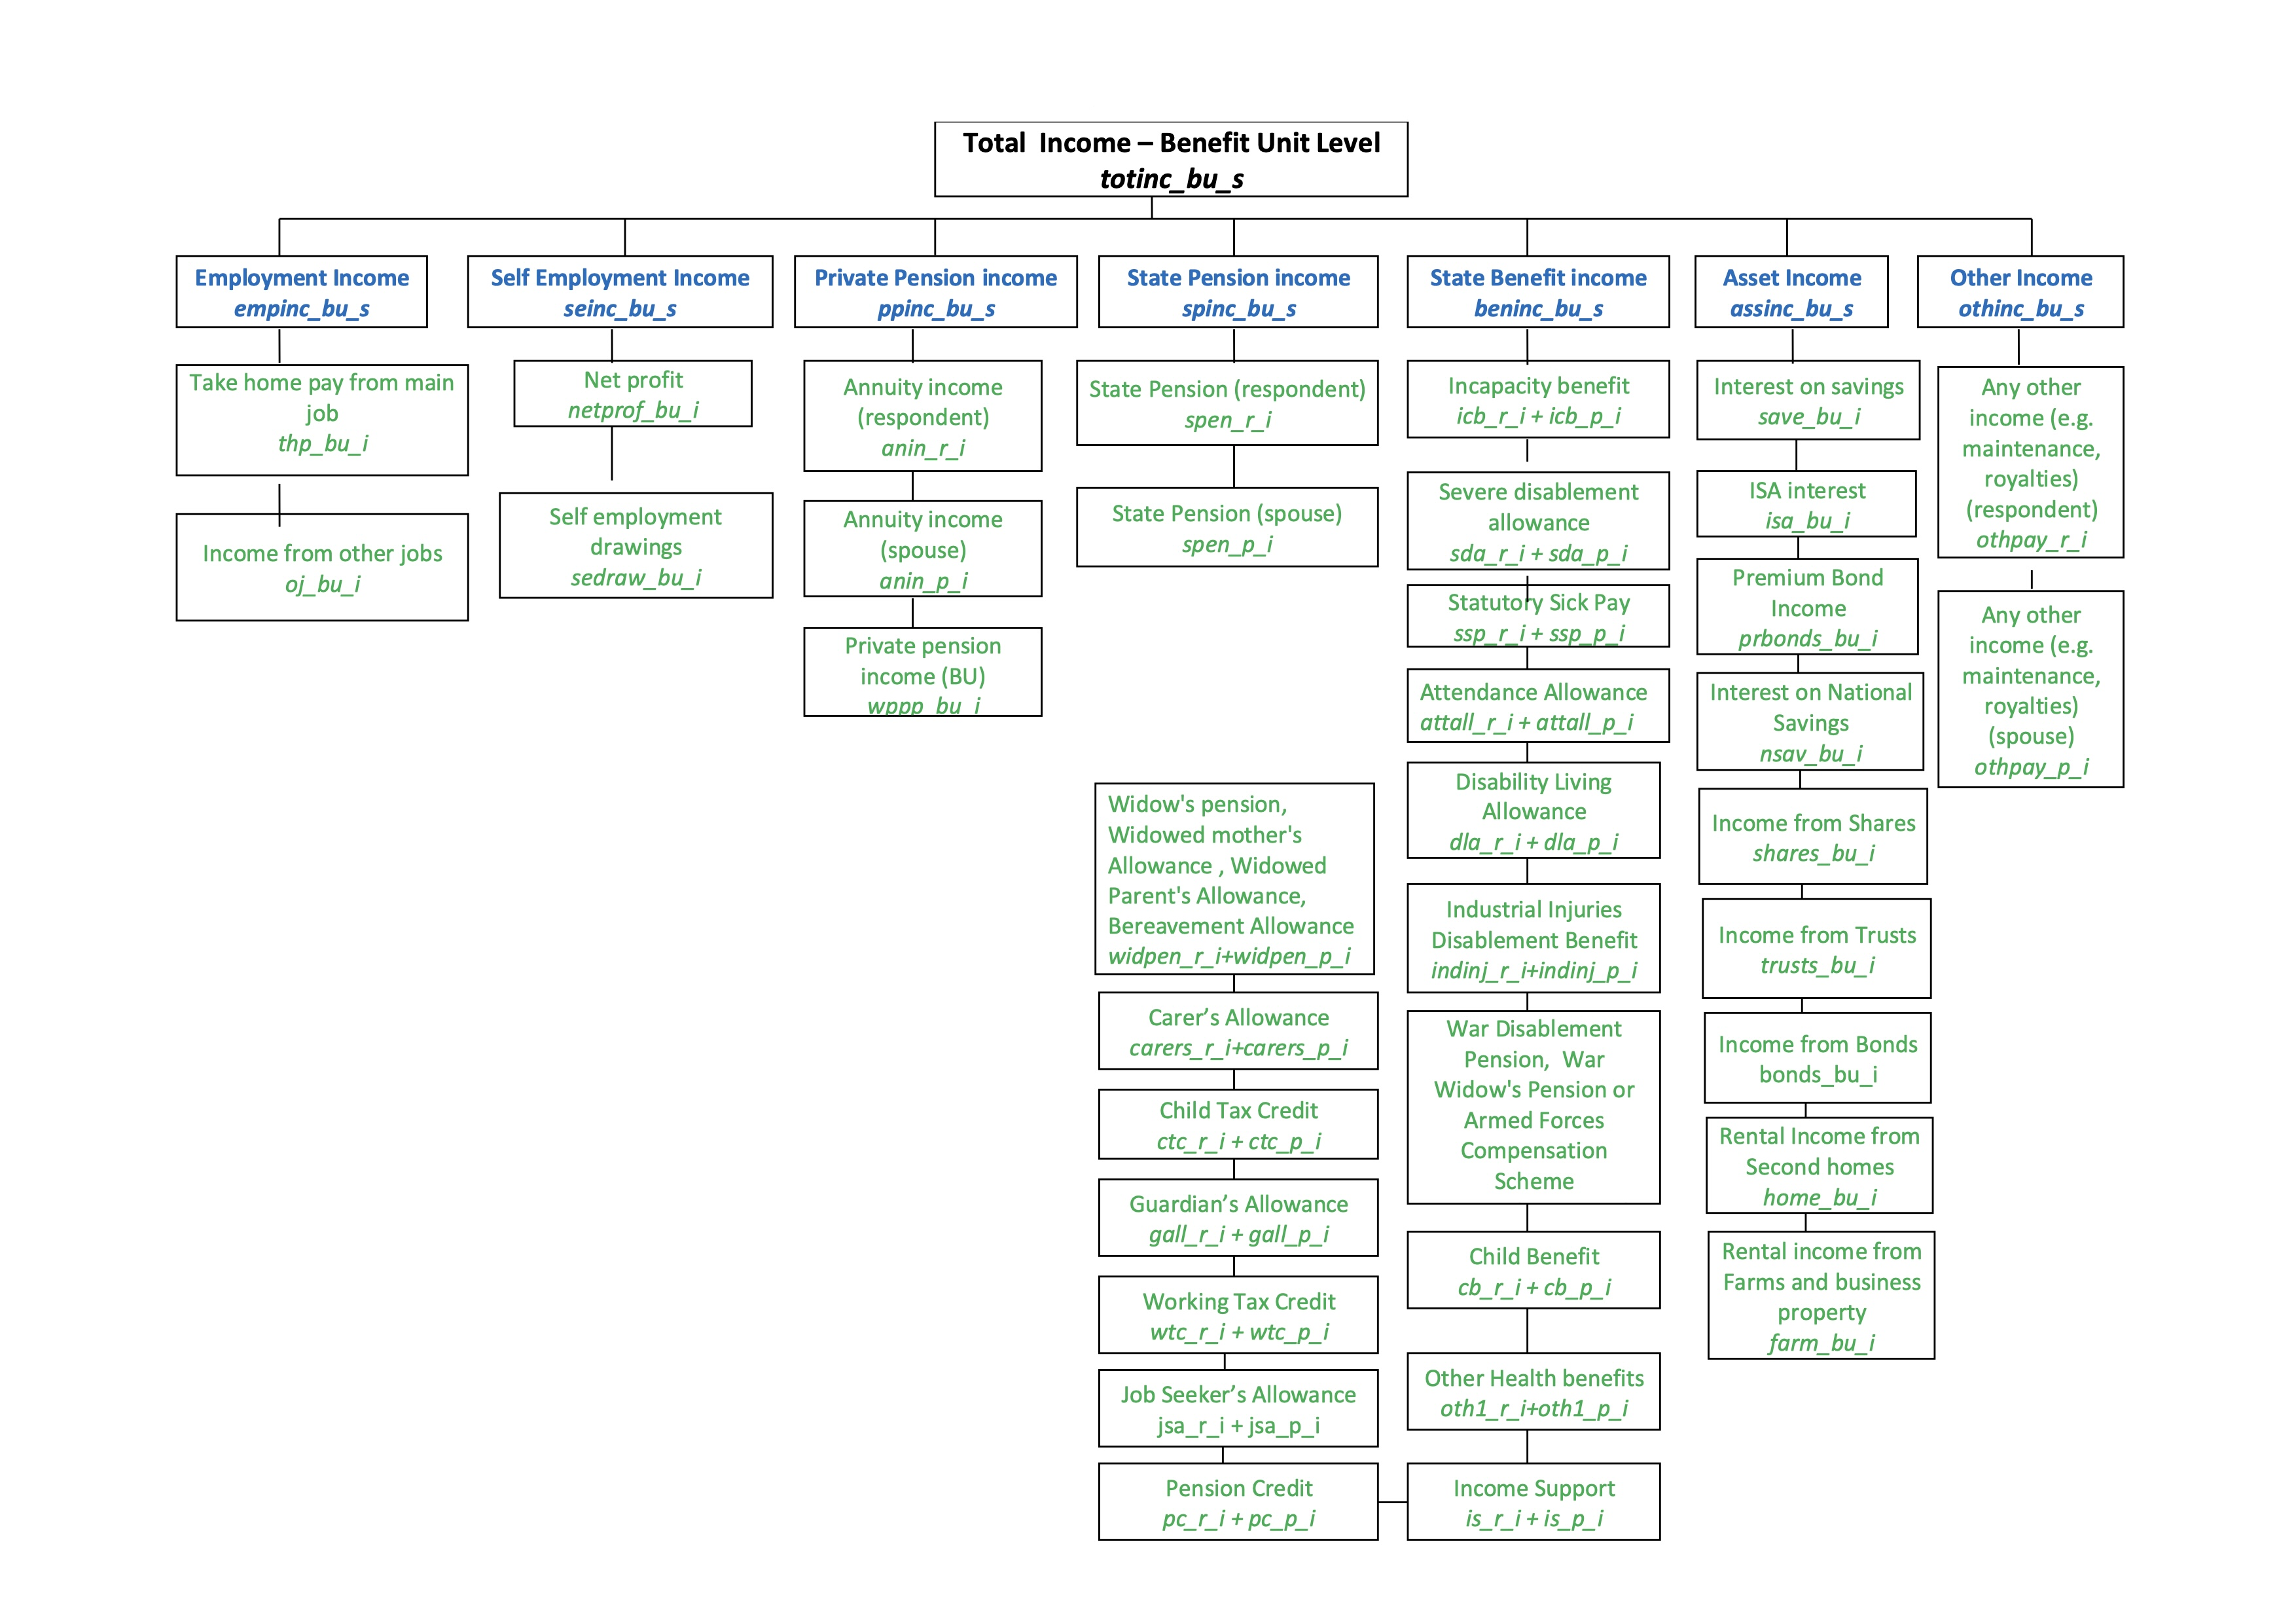
\includegraphics[width=0.8\textwidth]{figures/household_income.jpg}
    \end{figure}

    \item Deprivation \\
    Deprivation is measured through a series of nine questions that ask respondents whether they have any activities stopped by having too little money (see Table \ref{tab:deprivation} for a detailed list of questions). This study constructs a deprivation index based on the number of affirmative responses, with the index ranging from 0 (least deprived) to 9 (most deprived). For analysis purposes, this deprivation index is treated as a continuous variable.

    \begin{table}[h!]
        \centering
        \caption{Deprivation questions --- Activities stopped by having too little money}
        \label{tab:deprivation}
        \begin{tabularx}{\textwidth}{lX}
            \toprule 
            Item & Description \\
            \midrule
            1 & Buy your first choices of food items \\
            2 & Have family and friends round for a drink or meal \\
            3 & Have an outfit to wear for social or family occasions \\
            4 & Keep your home in a reasonable state of decoration \\
            5 & Replace or repair broken electrical goods \\
            6 & Pay for fares or other transport costs to get to and from places you want to go \\
            7 & Buy presents for friends or family once a year \\
            8 & Take the sorts of holidays you want \\
            9 & Treat yourself from time to time \\
            \bottomrule
        \end{tabularx}
    \end{table}

    \item Cognitive functioning \\
    Cognitive functioning is a multifaceted concept that encompasses the mental processes of perception, learning, memory, understanding, awareness, reasoning, judgment, intuition, and language (American Psychological Association, 2018). This study focuses on three aspects of cognitive functioning available in ELSA: \\
    Memory: Memory is measured through respondents' self-assessment on a five-point ordinal scale: 1 (excellent), 2 (very good), 3 (good), 4 (fair), 5 (poor). For analysis purposes, memory is treated as a continuous variable. \\
    Numeracy: Numeracy ability is evaluated using a series of seven questions that require respondents to sequentially subtract 7 from 100. This study calculates a numeracy index based on the number of correct responses, with the index ranging from 0 (lowest numeracy ability) to 7 (highest numeracy ability). This numeracy index is also treated as a continuous variable for analysis. \\
    Comprehension: Comprehension ability is assessed through a set of four questions where respondents are provided with an information card about a specific medicine called ``Medco”, and asked questions pertaining to its content (see Table \ref{tab:comprehension} for a detailed list of questions). This study calculates a comprehension index based on the number of correct responses, with the index ranging from 0 (lowest comprehension ability) to 4 (highest comprehension ability). This comprehension index is also treated as a continuous variable for analysis purposes. Notably, due to differences in survey design, the comprehension questions were only included in Wave 10. Consequently, the comprehension index is utilised solely for the first research question.

    \begin{table}[h!]
        \centering
        \caption{Comprehension ability questions}
        \label{tab:comprehension}
        \begin{tabular}{ll}
            \toprule
            Item & Description \\
            \midrule
            1 & What is the maximum number of days you may take this medicine \\
            2 & List three situations for which you should consult a doctor \\
            3 & List one condition for which you might take the Medco tablet \\
            4 & List one condition for which you should not take the Medco tablet \\
            \bottomrule
        \end{tabular}
    \end{table}

\end{itemize}

\section{Identification strategy - RQ1}
The first research question investigates the causal effect of digital literacy on older adults' health outcomes, using data from Wave 10 of ELSA. The explanatory variable is the dichotomised digital literacy index. Specifically, the treatment group contains respondents with high digital literacy (those above the median), while the control group contains respondents with low digital literacy (those below the median). The estimand of this research question is the Average Treatment Effect (ATE):

\begin{equation}
    \label{eq:ate}
    ATE = E(Y_i^1) - E(Y_i^0)
\end{equation}

As highlighted in Section 2.3.2, the relationship between digital literacy and health is complicated by two endogeneity issues: simultaneity bias and omitted variable bias. The identification strategy for the first research question aims to address both biases to derive a valid estimate of the effect of digital literacy on the health outcomes of older adults. 

\subsection{Addressing simultaneity bias}
As explored in Section 2.3.2, simultaneity bias (i.e., reverse causality) possibly exists in two scenarios: poorer health conditions can either decrease or increase levels of digital literacy.

The primary reason poorer health may lead to lower level of digital literacy is that health problems hinder the ability to learn or use the Internet. To address this issue, this study considers respondents' reasons behind their limited Internet usage. At Wave 10, ELSA includes a specific question about why respondents do not use the Internet more frequently (see Table \ref{tab:reverse_causality} for a detailed list of responses). To mitigate this aspect of simultaneity bias, this study excludes respondents who answered ``5” or ``6” to this question, effectively removing those for whom health problems is one of the factors that prevent Internet usage.

\begin{table}[h!]
    \centering
    \caption{Reasons why respondents do not use the Internet more}
    \label{tab:reverse_causality}
    \begin{tabular}{ll}
        \toprule
        Item & Reason \\
        \midrule
        1 & IT skills are not good enough \\
        2 & Don't trust the internet (fraud, sharing personal data) \\
        3 & Don't have good enough access to broadband \\
        4 & Don't have access to good enough equipment \\
        5 & Vision is not good enough to use the equipment \\ 
        6 & Health problems stop me from using the equipment \\ 
        7 & No reason to use it more \\
        8 & Takes too much time \\
        9 & None of the above \\
        \bottomrule
    \end{tabular}
\end{table}

The primary reason poorer health may lead to higher level of digital literacy is that mobility limitations necessitate the use of the Internet for everyday tasks. To address this issue, this study specifically targets and excludes respondents with such limitations. In ELSA, mobility is assessed based on the respondents' ability to walk a quarter of a mile without the aid of any special equipment. Respondents who are unable to walk this distance unaided are excluded from the analysis.

In summary, these two exclusions of respondents help ensure the remaining sample is not subject to simultaneity bias. This methodology offers a distinct advantage over much of the existing literature, which often fail to adequately address simultaneity bias. By addressing both scenarios of simultaneity bias, this study strengthens the validity of its estimate regarding the causal effect of digital literacy on health outcomes.

\subsection{Addressing omitted variable bias}
This study employs Inverse Probability of Treatment Weighting (IPTW), also known as the marginal structural model, to address omitted variable bias. The core concept in IPTW, ``probability of treatment”, is referred to as the “propensity score”, which is defined as a respondent's probability of receiving the treatment, regardless of the actual treatment status (Angrist \& Pischke, 2009, p. 80). 

Originally, the relationship between digital literacy (D) and health outcome (Y) is confounded by other variables (X). In the Directed Acyclic Graph (DAG) framework, this issue can be expressed as there is an unblocked backdoor path between D and Y (i.e., $D \leftarrow X \rightarrow Y$) (see Figure \ref{fig:backdoor}). 

\begin{figure}[h!]
    \centering
    \caption{Unblocked backdoor path}
    \label{fig:backdoor}
    \begin{tikzpicture}[thick]
        \node (D) {D};
        \node (X) [below right = of D] {X};
        \node (Y) [above right = of X] {Y};
          
        \draw[->] (X) -- (D);
        \draw[->] (X) -- (Y);
        \draw[->] (D) -- (Y);
      \end{tikzpicture}
\end{figure}

IPTW corrects for this by weighting respondents by the inverse of their propensity score. This method creates a pseudo-sample where D is independent of Z, allowing for a direct estimation of the effect of D on Y (see Figure \ref{fig:blocked}). In the DAG framework, IPTW manages to eliminate the backdoor path between D and Y. It has been mathematically demonstrated that when the propensity score is accurately specified, IPTW provides an unbiased and consistent estimate of the actual treatment effect (Lunceford \& Davidian, 2004).

\begin{figure}[h!]
    \centering
    \caption{Blocked backdoor path}
    \label{fig:blocked}
    \begin{tikzpicture}[thick]
        \node (D) {D};
        \node (X) [below right = of D] {X};
        \node (Y) [above right = of X] {Y};
          
        \draw[->] (X) -- (Y);
        \draw[->] (D) -- (Y);
      \end{tikzpicture}
\end{figure}

The specific process of implementing IPTW is as follows:

\begin{enumerate}[wide=0pt, leftmargin=*, labelwidth=0pt, labelindent=\parindent, itemindent=0pt]
    \item Estimate propensity score \footnote{Apart from the logistic model employed in this study, the probit model is also commonly used in the literature for estimating propensity scores (Abadie \& Imbens, 2016). To validate the robustness of this study's findings and to ensure they are not influenced by the specific choice of statistical model, the analysis is repeated with propensity scores estimated from the probit model. The results derived from both models were largely identical (see Appendix for details on the probit model analysis).} \\
    Propensity scores are estimated using a logistic model (see Equation \ref{eq:logit_rq1}) that regresses respondents' actual treatment status (D) on the twelve control variables (\textbf{X}) listed in Section 4.3.3. Propensity scores correspond to the fitted values from this logistic model (see Equation \ref{eq:propensity_score_rq1}).

    \begin{equation}
        \label{eq:logit_rq1}
        Logit(D) \sim \textbf{X}
    \end{equation}

    \begin{equation}
        \label{eq:propensity_score_rq1}
        \textnormal{Propensity score} = \hat{P}(D = 1 | \textbf{X})
    \end{equation}

    \item Compute weights \\
    As the estimand of the study is ATE, the weights are calculated as the inverse of the probability that respondents received the treatment they actually received (see Equation \ref{eq:raw_weights}).

    \begin{equation}
        \label{eq:raw_weights}
        \begin{aligned}
            \textnormal{For } D &= 1: \textnormal{weight} = \frac{1}{\hat{P}(D = 1 | \textbf{X})} \\
            \textnormal{For } D &= 0: \textnormal{weight} = \frac{1}{1 - \hat{P}(D = 1 | \textbf{X})}
        \end{aligned}
    \end{equation}

    However, using these unstabilised weights can lead to two significant issues. Firstly, since the propensity score ranges between 0 and 1, the resulting weights ($\frac{1}{\textnormal{propensity score}}$) for each respondent will always exceed 1, leading to an artificially inflated sample size in the pseudo-sample compared to the original sample (Morgan \& Winship, 2014, p. 413). Secondly, treated respondents with very low propensity scores will have considerably large weights. Similarly, control respondents with propensity scores close to one also receive large weights. Such disproportionate weights can increase the variance and widen the confidence intervals, potentially distorting the study's findings (Cole \& Hernan, 2008).

    To mitigate these issues, it is more recommended to use stabilised weights, which involve multiplying the unstabilised weights by the expected value of the treatment ($E(D = d)$) (see Equation \ref{eq:stabilisied_weights}). With stabilised weights, the pseudo sample size remains consistent with the original sample, and the variance is not artificially inflated, ensuring a more robust and reliable analysis (Morgan \& Winship, 2014, p. 413).

    \begin{equation}
        \label{eq:stabilisied_weights}
        \begin{aligned}
            \textnormal{For } D &= 1: \textnormal{weight} = \frac{E[D = 1]}{\hat{P}(D = 1 | \textbf{X})} \\
            \textnormal{For } D &= 0: \textnormal{weight} = \frac{E[D = 0]}{1 - \hat{P}(D = 1 | \textbf{X})}
        \end{aligned}
    \end{equation}

    \item Run a weighted regression \\
    Finally, a weighted Ordinary Least Squares (OLS) regression is conducted, where the health outcome (Y) is regressed against digital literacy (D) using the stabilised weights derived earlier. The ATE, the outcome of interest of the first research question, corresponds to the coefficient of digital literacy. Eight separate OLS models are constructed for each health outcome, encompassing one model for self-rated health, six for physical health conditions, and one for mental health. 

    Although the outcome variables for physical and mental health are binary, OLS regression is used for its straightforward parametric characteristics and ease of interpretation. This approach aligns with the primary objective of the study, which is to identify the true causal effect rather than delineate the precise functional relationships between the variables. Nevertheless, to further validate the robustness of the findings, a series of logistic regression analyses for the binary health outcomes are also conducted. Results from these models are presented in Appendix. Findings from both OLS and logistic regression analysis are largely consistent, which reinforces the robustness and reliability of the conclusions.
\end{enumerate}

Two critical assumptions must be satisfied for the IPTW results to be considered an unbiased estimate of the true causal effect. The first assumption is strong ignorability, which posits that the estimated propensity score should represent the true propensity score. This requires the propensity score model should incorporate all variables that influence the treatment selection process. If unmeasured confounders exist, the assumption of strong ignorability is violated, and the estimate may be biased (Cole \& Hernan, 2008). The strong ignorability assumption is untestable as one cannot empirically verify whether all possible confounders have been included. 

The second assumption is the positivity assumption, which asserts that there are both treated and untreated individuals present at every level of the confounders. A violation of this assumption occurs when certain combinations of covariate levels inherently prevent respondents from receiving treatment, leading to what is termed "structural zeros" (Austin \& Stuart, 2015). Theoretically, this assumption is testable in the sense that one could examine whether any part of the covariate distribution exclusively contains treated or untreated respondents. However, practical failures of this test do not necessarily indicate a violation because such failures might instead result from "random zeros", where absence of treated respondents is due to chance rather than structural impediments (Cole \& Hernan, 2008). The complexity of ensuring positivity increases significantly with the number of covariates due to the ``curse of dimensionality". In such scenarios, some levels of covariates might inevitably appear to be exclusively treated or untreated, not necessarily because these covariate levels prevent treatment, but rather due to the sparse distribution of data across high-dimensional space (Morgan \& Winship, 2014, p. 397).

\section{Robustness checks - RQ1}
Following the discussion above, the validity of the IPTW results hinges on the satisfaction of the strong ignorability and positivity assumptions. To assess the robustness of these assumptions, this section will discuss empirical methods to assess their plausibility in this study.

The strong ignorability assumption is inherently untestable because it is impossible to confirm whether all potential confounders have been accounted for. However, sensitivity analysis offers a method to estimate how large the effect of an unmeasured confounder would need to be to negate the observed relationship between digital literacy (D) and health outcomes (Y) (Shen et al., 2011). Consider the following DAG where X represents one of the controlled confounders and U represents an unmeasured confounder. Assume the true effect of U on D is $\delta$, the true effect of U on Y is $\gamma$, and the estimated effect of D on Y is $\hat{\beta}$.

\begin{figure}[h!]
    \centering
    \caption{Illustration of sensitivity analysis}
    \label{fig:sense_dag}
    \begin{tikzpicture}[thick]
        \node (D) {D};
        \node (X) [below right = of D] {X};
        \node (Y) [above right = of X] {Y};
        \node (U) [above right = of D] {U};
          
        \draw[->] (X) -- (D);
        \draw[->] (X) -- (Y);
        \draw[->] (D) -- (Y) node[midway, above] {$\hat{\beta}$};
        \draw[->] (U) -- (D) node[midway, above] {$\delta$};
        \draw[->] (U) -- (Y) node[midway, above] {$\gamma$};
      \end{tikzpicture}
\end{figure}

The omitted variable bias here is $\delta \times \gamma$. The fundamental idea of sensitivity analysis is to investigate how large this bias has to be in order to nullify the observed effect of D on Y. This is operationalised through pick hypothetical values of $\delta$ and $\gamma$ and see how sensitive $\hat{\beta}$ is to them. While any values could theoretically be chosen for $\delta$ and $\gamma$, it is practical to benchmark these against the effects of a known confounder X. Specifically, this involves comparing the effect of U on D (i.e., $\delta$) against the effect of X on D, and comparing the effect of U on Y (i.e., $\gamma$) against the effect of X on Y (VanderWeele \& Ding, 2017). 

This study selects ``deprivation” as the controlled confounder $X$, against which the impact of the uncontrolled confounder $U$ will be assessed. Deprivation is particularly apt for this role, as it is extensively documented in the literature and is one of the most significant confounders in terms of its effect size on the relationship between digital literacy and health (Hall et al., 2015; He et al., 2022). It notably influences older adults' health conditions and their digital literacy levels directly and substantially. 

This comparative method provides an intuitive assessment of the potential influence of uncontrolled confounders. If the analysis reveals that exceedingly large values of $\delta$ and $\gamma$ are required to nullify the observed relationship between D and Y — essentially, if this relationship could only be negated by an uncontrolled confounder whose impact on D and Y is significantly greater than that of deprivation — this would suggest it is highly improbable to encounter an uncontrolled confounder with such disproportionately large effects (Shen et al., 2011). Such findings will greatly enhance the robustness of this study's conclusions against potential violations of the strong ignorability assumption. Conversely, if it is discovered that relatively small effects from an uncontrolled confounder could negate the observed relationship, this would indicate a vulnerability in the findings and necessitate a reconsideration of the robustness of the causal inference drawn from the study.

Regarding the positivity assumption, as elaborated in Section 4.4.2, while this assumption is in theory testable, occurrences of exclusively treated or untreated covariate levels may arise due to ``structural zeros" (indicating a true violation of the positivity assumption) or ``random zeros" (attributable to the ``curse of dimensionality" and not constituting a true violation). Considering the inclusion of 12 covariates in the propensity score estimation, such tests may not always be effective. Therefore, following the two rules of thumb proposed by Cole and Hernan (2008), this study i) calculates the mean of the stabilised weights, and ii) obtains the minimum and maximum values of the stabilised weights. If the mean deviates significantly from one, or if the minimum and maximum values are too extreme, this will indicate a potential violation of the positivity assumption. 

\section{Identification strategy - RQ2}
The second research question investigates whether increased digitalisation will exacerbate the existing health inequalities between older adults with low and high levels of digital literacy. This study draws on the exogenous increase in digitalisation triggered by the COVID-19 pandemic (Pandit et al., 2022; Spanakis et al., 2021). ELSA's Wave 9 was conducted pre-pandemic (from June 2018 to July 2019), while Wave 10 was conducted during the pandemic (from October 2021 to July 2022) (NatCen Social Research, 2020, 2022). This temporal distinction provides an ideal setting to investigate the impact of increased digitalisation on health inequalities. Specifically, the treatment in this research question is the increased digitalisation occurred between Wave 9 and 10, and the two comparison groups are respondents with low and high digital literacy according to the dichotomised digital literacy index.

As highlighted in Section 2.4.2, applying a simple Difference-in-Difference (DiD) design will not achieve the desired result as DiD has two potential drawbacks in this context. The identification strategy for the second research questions aims to address both drawbacks to derive a valid estimate of the impact of increased digitalisation on the health inequalities between older adults with low and high levels of digital literacy.

\subsection{Addressing contamination of group assignment}
As discussed in Section 2.4.2, digital literacy is not a static attribute. Changes in respondents' digital literacy between waves may lead to potential contamination of group assignments, thereby biasing the analysis results. To mitigate this issue, this study conducts separate PCAs for Wave 9 and Wave 10 to derive digital literacy index for each wave, which are then dichotomised based on median cutoff respectively. For the analysis of the second research question, only respondents whose digital literacy levels remain consistent across the two waves (i.e., either always low or always high) are included in the analysis. This further sample selection should be able to minimise the impact of group assignment contamination caused by digital literacy fluctuations.

\subsection{Addressing possible violations of parallel trends assumption}
This study employs a combined Propensity Score Matching and Difference-in-Difference approach, also known as Matching DiD, to address potential violations of the parallel trends assumption. As discussed in Section 2.4.2, inherent heterogeneity between the two groups, such as the difference in educational attainment, may already predispose their health trends to diverge irrespective of any change in digitalisation (Hall et al., 2015). The core concept of Matching DiD involves a strategic refinement of the traditional DiD approach: Rather than applying DiD analysis to the entire sample, Matching DiD starts by matching respondents in the low digital literacy group with a very ``similar” counterpart in the high digital literacy group. This similarity is defined by the expectation that, respondents with more similar characteristics are more likely to demonstrate parallel health trends in the absence of any digitalisation changes (Pufahl \& Weiss, 2009). Once these similar pairs are identified, separate DiD analyses are conducted on each pair, and the results are then aggregated to form the final estimate (Dehejia \& Wahba, 1999).

The effectiveness of Matching DiD centres on the accurate selection of "similar" respondents. To achieve this, it is important to match on variables which the two groups significantly differ in and influence their health trends. These variables mirror the confounders identified for the first research question, as they both represent variables that are correlated with both digital literacy and health. Consequently, this study employs the eleven control variables \footnote{As mentioned in Section 4.3.3, comprehension ability is not included in the second research question because it is not measured in Wave 9.} described in Section 4.3.3 as the matching covariates.

The specific matching DiD process is as follows:

\begin{enumerate}[wide=0pt, leftmargin=*, labelwidth=0pt, labelindent=\parindent, itemindent=0pt]
    \item Estimate propensity score \footnote{Similarly as Section 4.4.2, to ensure the robustness of this study's findings, the analysis is repeated with propensity scores estimated from the probit model. The results derived from both models were largely identical (see Appendix for details on the probit model analysis).} \\
    Propensity scores are estimated using a logistic model (see Equation \ref{eq:logit_rq2}) that regresses respondents' group assignment (i.e. low or high digital literacy) on the eleven control variables (\textbf{X}) listed in Section 4.3.3. Propensity scores correspond to the fitted values from this logistic model (see Equation \ref{eq:propensity_score_rq2}).

    \begin{equation}
        \label{eq:logit_rq2}
        Logit(D) \sim \textbf{X}
    \end{equation}
    
    \begin{equation}
        \label{eq:propensity_score_rq2}
        \textnormal{Propensity score} = \hat{P}(D = 1 | \textbf{X})
    \end{equation}

    \item Conduct matching based on propensity scores \\
    The matching method employed is K-Nearest Neighbour (KNN) matching, with the number of neighbours (K) set to one (i.e. match one respondent in the low digital literacy group to one respondent in the high digital literacy group). Matching is conducted with replacement, and the distance between two respondents is determined by the Euclidean distance of their propensity scores.  

    To further verify the robustness of the matching process, this study explores various combinations of matching parameters such as the number of neighbours (K), and matching with or without replacement. The results from these different parameter settings are detailed in Appendix and demonstrate a high degree of consistency, thereby confirming the robustness of the findings across different matching configurations.

    \item Calculate DiD within each matched pair \\
    Finally, DiD is performed within each matched pair. This involves firstly calculating the difference in health outcomes between Wave 9 and Wave 10 for each respondent, and subsequently calculating the differences between the two matched respondents in each pair. This process results in a distribution of DiD estimates across all matched pairs. From this distribution, the mean is calculated, providing the final estimate of the impact of increased digitalisation on health disparities between respondents with low and high digital literacy (see Equation \ref{eq:did}). Additionally, the standard deviation of these differences is computed to facilitate further statistical inference and analysis of the results.

    \begin{equation}
        \label{eq:did}
        \delta_{DiD} = \sum_{i=1}^{n} \left( (Y_{i}^{10high} - Y_{i}^{9high}) - (Y_{i}^{10low} - Y_{i}^{9low}) \right)
    \end{equation}
    where i represents matched pairs
\end{enumerate}

It is important to acknowledge that combining PSM with DiD does not completely eliminate concerns regarding the parallel trends assumption, which is inherently untestable. The fundamental approach here is to meticulously match respondents who are as similar as possible. The more similar the characteristics of these pairs, the higher the likelihood that the parallel trends assumption will hold. Although Matching DiD does not provide a perfect solution, it significantly enhances the likelihood of achieving a more accurate comparison between the groups. Therefore, it is reasonable to argue that, compared to the simple DiD approach, the estimates derived from the Matching DiD approach offer a more refined understanding of how increased digitalisation affects the health disparities between older adults with low and high levels of digital literacy.